\documentclass[
  coursetitle={Cómputo Nube y Tecnologías Emergentes},
  coursehours={96},
  coursedate={Verano 2026},
  doctype={Tutorial},
  otherlangs={english,french},
  authorname={Lázaro},
  authorsurname={Bustio-Martínez},
  authortitle={PhD},
  role={Profesor Investigador},
  email={lbustio@inaoe.mx},
  phone={5559504000},
  ext={7459},
  institution={Instituto Nacional de Astrofísica, Óptica y Electrónica (INAOE)},
  department={Maestría en Ciencias en Tecnologías de Seguridad},
  address={Luis Enrique Erro 1, Sta. Ma. Tonantzintla, San Andrés Cholula, CP 72840, Puebla, México},
  margin={0.5in}
]{../../lbustio_lecture_notes}

\usepackage[utf8]{inputenc}
\usepackage[T1]{fontenc}
\usepackage{array}
\usepackage{tabularx}
\usepackage{enumitem}
\usepackage{longtable}
\usepackage{booktabs}
\usepackage{url}
\usepackage{listings}
\usepackage{xcolor}
\usepackage{graphicx}
\usepackage{tcolorbox}
\usepackage{verbatim}
\usepackage{tikz}
\usetikzlibrary{arrows.meta,backgrounds,fit,positioning}

\definecolor{lightgray}{rgb}{0.97, 0.97, 0.97}
\definecolor{darkblue}{rgb}{0, 0, 0.6}
\definecolor{gcpblue}{HTML}{4285F4}
\definecolor{gcpgreen}{HTML}{34A853}
\definecolor{gcpyellow}{HTML}{FBBC04}
\definecolor{gcpred}{HTML}{EA4335}
\definecolor{softgray}{HTML}{F5F7FA}
\definecolor{androidgreen}{HTML}{3DDC84}
\definecolor{androiddark}{HTML}{073042}

\lstset{
  backgroundcolor=\color{lightgray},
  basicstyle=\ttfamily\small,
  breaklines=true,
  frame=single,
  columns=fullflexible,
  showstringspaces=false,
  commentstyle=\color{gray},
  keywordstyle=\color{darkblue},
  inputencoding=utf8,
  extendedchars=true,
  literate={á}{{\'a}}1 {é}{{\'e}}1 {í}{{\'i}}1 {ó}{{\'o}}1 {ú}{{\'u}}1 {ñ}{{\~n}}1
           {Á}{{\'A}}1 {É}{{\'E}}1 {Í}{{\'I}}1 {Ó}{{\'O}}1 {Ú}{{\'U}}1 {Ñ}{{\~N}}1
}

\setlist[itemize]{topsep=0.3em,itemsep=0.2em}
\setlist[enumerate]{topsep=0.3em,itemsep=0.2em}

\tikzset{
  apkstage/.style={
    draw=androiddark,
    fill=androiddark!7,
    rounded corners=4pt,
    very thick,
    align=center,
    text width=0.62\textwidth,
    minimum height=1.15cm,
    inner sep=7pt
  },
  apkstage2/.style={
    apkstage,
    draw=androidgreen!80!black,
    fill=androidgreen!9
  },
  apkstage3/.style={
    apkstage,
    draw=gcpblue,
    fill=gcpblue!7
  },
  apkstage4/.style={
    apkstage,
    draw=gcpred,
    fill=gcpred!7
  },
  compactapk/.style={
    draw=androiddark,
    fill=softgray,
    rounded corners=4pt,
    thick,
    align=center,
    text width=3.2cm,
    minimum height=1.0cm,
    inner sep=5pt
  },
  flowarrow/.style={
    -{Latex[length=3mm,width=2mm]},
    thick,
    draw=darkblue
  }
}

\begin{document}

\IberoCover

\section{Objetivo de la práctica}

El objetivo de esta práctica es responder una pregunta de investigación concreta mediante análisis estático y aprendizaje automático: ¿los permisos declarados en el manifiesto de una aplicación Android contienen información suficiente para clasificarla automáticamente como benigna o maliciosa?

Al finalizar la práctica, el estudiante será capaz de:

\begin{itemize}
    \item representar aplicaciones Android como vectores binarios de permisos;
    \item realizar un análisis exploratorio orientado a comparar dos clases de aplicaciones;
    \item identificar permisos frecuentes, diferenciales y sensibles;
    \item minar itemsets frecuentes y generar reglas de asociación y clasificación;
    \item aplicar pruebas estadísticas para contrastar hipótesis;
    \item entrenar y evaluar modelos de clasificación supervisada;
    \item interpretar matrices de confusión, curvas ROC y la importancia de características;
    \item guardar y reutilizar un modelo entrenado;
    \item consumir el modelo desde una interfaz web y desde la línea de comandos.
\end{itemize}

\section{Planteamiento del problema}

El ecosistema Android permite instalar aplicaciones desde múltiples fuentes, lo que incrementa la exposición de los usuarios a APKs potencialmente maliciosas. Antes de ejecutar una aplicación, una fuente de información disponible es el conjunto de permisos declarados en su archivo \texttt{AndroidManifest.xml}.

Sin embargo, los permisos presentan un problema de solapamiento: muchas aplicaciones benignas también solicitan permisos sensibles para cumplir funciones legítimas. Por ello, no es evidente si los permisos declarados son suficientes para distinguir automáticamente entre APKs benignas y maliciosas.

\textbf{Pregunta de investigación:} ¿Los permisos declarados por las aplicaciones Android contienen información discriminativa suficiente para clasificar APKs como benignas o maliciosas, y qué diferencias existen entre ambas clases en cuanto a cantidad, tipo y distribución de permisos solicitados?

\subsection{Hipótesis}

\begin{description}
    \item[H1.] Los permisos declarados contienen información suficiente para que los modelos supervisados superen una línea base trivial.
    \item[H2.] Las APKs maliciosas solicitan, en promedio, más permisos que las benignas.
    \item[H3.] Las APKs maliciosas solicitan con mayor frecuencia permisos sensibles.
    \item[H4.] Existe solapamiento entre permisos de ambas clases, pero la distribución de frecuencias difiere entre ellas.
    \item[H5.] La combinación de permisos tiene mayor capacidad predictiva que el análisis de permisos individuales.
    \item[H6.] Un subconjunto reducido de permisos permite obtener un desempeño comparable al conjunto completo.
\end{description}

\section{Arquitectura de la solución}

La práctica sigue un flujo de análisis estático reproducible. Los datos provienen de un dataset de APKs etiquetadas; el análisis ocurre en un notebook Jupyter; el modelo resultante se integra en una aplicación web que acepta archivos APK reales.

\begin{center}
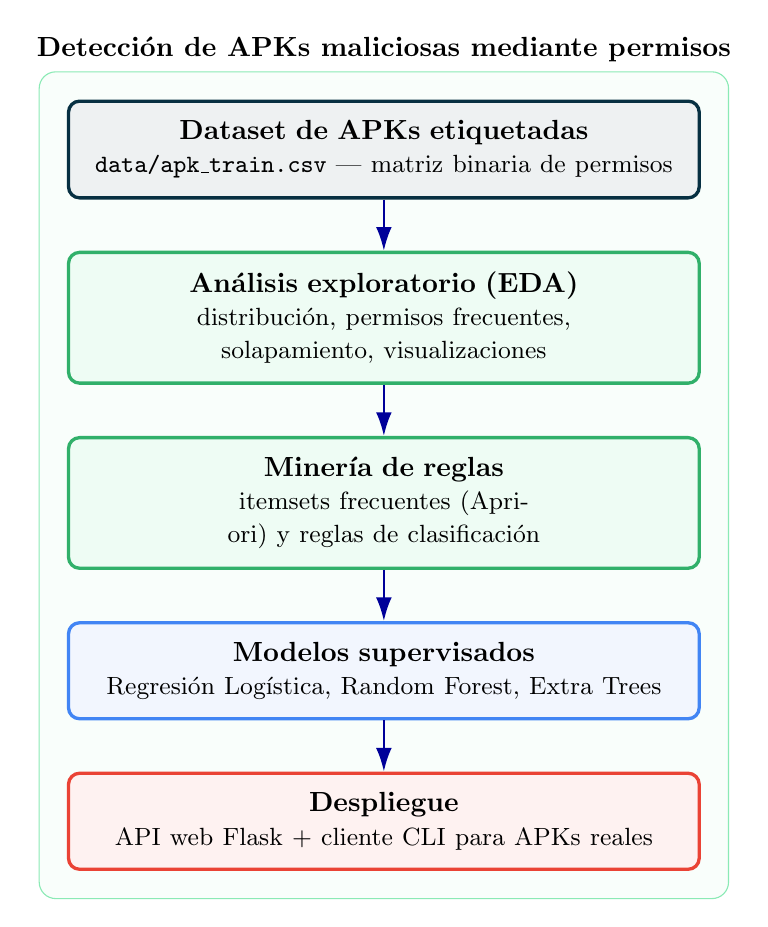
\begin{tikzpicture}[node distance=0.65cm]
    \node[apkstage] (datos) {
        \textbf{Dataset de APKs etiquetadas}\\
        \small \texttt{data/apk\_train.csv} --- matriz binaria de permisos
    };
    \node[apkstage2, below=of datos] (eda) {
        \textbf{Análisis exploratorio (EDA)}\\
        \small distribución, permisos frecuentes, solapamiento, visualizaciones
    };
    \node[apkstage2, below=of eda] (reglas) {
        \textbf{Minería de reglas}\\
        \small itemsets frecuentes (Apriori) y reglas de clasificación
    };
    \node[apkstage3, below=of reglas] (modelos) {
        \textbf{Modelos supervisados}\\
        \small Regresión Logística, Random Forest, Extra Trees
    };
    \node[apkstage4, below=of modelos] (despliegue) {
        \textbf{Despliegue}\\
        \small API web Flask + cliente CLI para APKs reales
    };

    \draw[flowarrow] (datos) -- (eda);
    \draw[flowarrow] (eda) -- (reglas);
    \draw[flowarrow] (reglas) -- (modelos);
    \draw[flowarrow] (modelos) -- (despliegue);

    \begin{scope}[on background layer]
        \node[
            draw=androidgreen!60,
            fill=androidgreen!3,
            rounded corners=6pt,
            inner sep=10pt,
            fit=(datos)(eda)(reglas)(modelos)(despliegue),
            label={[font=\bfseries]above:Detección de APKs maliciosas mediante permisos}
        ] {};
    \end{scope}
\end{tikzpicture}

\small\textbf{Figura:} Flujo completo del análisis desde los datos hasta el despliegue.
\end{center}

\section{Tecnologías utilizadas}

\begin{description}
    \item[Python 3.11+.] Lenguaje base del proyecto.
    \item[Pandas.] Carga, limpieza y manipulación de la matriz de permisos.
    \item[NumPy.] Operaciones matriciales y estadísticas auxiliares.
    \item[Scikit-Learn.] Modelos supervisados, métricas de evaluación y validación cruzada.
    \item[SciPy.] Prueba estadística Mann-Whitney para contraste de hipótesis.
    \item[Matplotlib y Seaborn.] Visualizaciones del análisis exploratorio.
    \item[joblib.] Serialización y carga del modelo entrenado.
    \item[Flask.] Aplicación web para análisis de APKs reales.
    \item[JupyterLab.] Entorno interactivo para el notebook de análisis.
\end{description}

\section{Estructura del proyecto}

\begin{lstlisting}
malware_apk_detection/
  backend/
    android_threat_analyzer/
      manifest.py        # parser propio de AXML binario
      model.py           # entrenamiento, seleccion y prediccion
      analysis.py        # flujo de analisis y respuestas
      web.py             # rutas Flask
      config.py          # rutas y variables de entorno
      logging_config.py  # configuracion de logs
  frontend_cli/
    train_model.py       # entrenamiento por consola
    predict_apk.py       # prediccion por consola
  frontend_webapp/
    app.py               # punto de entrada Flask
    templates/index.html # interfaz web
    static/              # JavaScript y CSS
  data/
    apk_train.csv        # dataset (separador ;)
  models/
    android_permission_best_model.joblib
  notebooks/
    deteccion_apks_maliciosas_permisos.ipynb
  biblio/permission/
    investigacion.md     # planteamiento e hipotesis
  references/            # PDFs de referencia academica
  testapk/               # APKs para pruebas
\end{lstlisting}

\section{Preparación del entorno}

Active el entorno conda del proyecto:

\begin{lstlisting}
conda activate apk-malware
\end{lstlisting}

Abra el notebook desde la carpeta raíz del proyecto:

\begin{lstlisting}
jupyter lab notebooks/deteccion_apks_maliciosas_permisos.ipynb
\end{lstlisting}

En la primera celda de código, el notebook importa todas las dependencias necesarias:

\begin{lstlisting}
import joblib
import matplotlib.pyplot as plt
import numpy as np
import pandas as pd
import seaborn as sns
from pathlib import Path
from scipy.stats import mannwhitneyu
from sklearn.cluster import KMeans, AgglomerativeClustering
from sklearn.decomposition import PCA
from sklearn.dummy import DummyClassifier
from sklearn.ensemble import RandomForestClassifier, ExtraTreesClassifier
from sklearn.linear_model import LogisticRegression
from sklearn.manifold import TSNE
from sklearn.metrics import (
    accuracy_score, classification_report,
    confusion_matrix, roc_auc_score
)
from sklearn.model_selection import (
    cross_validate, StratifiedKFold, train_test_split
)
from sklearn.pipeline import Pipeline
from sklearn.preprocessing import StandardScaler
\end{lstlisting}

La configuración inicial define las rutas del proyecto y los parámetros reproducibles:

\begin{lstlisting}
DATA_PATH  = Path("../data/apk_train.csv")
MODELS_DIR = Path("../models")
TARGET     = "type"
RANDOM_STATE = 42
MIN_ITEMSET_SUPPORT = 0.03
MAX_ITEMSET_LEN     = 4
\end{lstlisting}

\begin{tcolorbox}[title=Semilla aleatoria]
Fijar \texttt{random\_state=42} garantiza que las particiones, el entrenamiento y los algoritmos estocásticos produzcan los mismos resultados en cada ejecución. Esto es imprescindible para reproducibilidad.
\end{tcolorbox}

\section{Carga y validación inicial del dataset}

Cargue el dataset. El separador es punto y coma:

\begin{lstlisting}
df_raw = pd.read_csv(DATA_PATH, sep=";")
df_raw.head()
\end{lstlisting}

Cada fila representa una APK y cada columna, salvo \texttt{type}, representa un permiso. Los valores son binarios: \texttt{1} indica que la APK declara ese permiso, \texttt{0} que no lo declara.

Revise las dimensiones y la calidad de los datos:

\begin{lstlisting}
print(f"Filas:                {df_raw.shape[0]:,}")
print(f"Columnas:             {df_raw.shape[1]:,}")
print(f"Permisos candidatos:  {df_raw.shape[1] - 1:,}")
print(f"Valores faltantes:    {df_raw.isna().sum().sum():,}")
print(f"Registros duplicados: {df_raw.duplicated().sum():,}")

df_raw[TARGET].value_counts().rename(
    index={0: "benigna", 1: "maliciosa"}
)
\end{lstlisting}

\textbf{Resultado esperado:} 398 APKs, 331 columnas, 330 permisos candidatos. La distribución inicial es balanceada: 199 APKs benignas (clase 0) y 199 maliciosas (clase 1).

\begin{tcolorbox}[title=Interpretación]
El balance entre clases facilita la evaluación: ningún modelo puede obtener un resultado alto simplemente prediciendo siempre la clase dominante. Esto nos permite usar accuracy como métrica de referencia sin sesgo de clase.
\end{tcolorbox}

\section{Limpieza y construcción de la matriz de permisos}

Elimine duplicados exactos, depure valores faltantes y convierta todas las columnas a tipo entero binario:

\begin{lstlisting}
df = df_raw.copy()
df = df.drop_duplicates().dropna().reset_index(drop=True)

permission_cols = [col for col in df.columns if col != TARGET]

for col in permission_cols + [TARGET]:
    df[col] = pd.to_numeric(df[col], errors="coerce")

df = df.dropna().reset_index(drop=True)
df[permission_cols + [TARGET]] = df[permission_cols + [TARGET]].astype(int)

X = df[permission_cols]
y = df[TARGET]

print(f"APKs tras limpieza: {len(df)}")
print(y.value_counts().rename(index={0: "benigna", 1: "maliciosa"}))
\end{lstlisting}

\textbf{Resultado esperado:} 224 APKs tras eliminar 174 duplicados exactos. La distribución queda en 114 benignas y 110 maliciosas.

\begin{tcolorbox}[title=Por qué eliminar duplicados]
Los duplicados pueden inflar artificialmente el desempeño de los modelos si una misma APK aparece tanto en entrenamiento como en prueba. Eliminarlos antes de particionar evita esta fuga de información.
\end{tcolorbox}

\section{Análisis exploratorio de datos}

\subsection{Distribución de clases}

Visualice el balance de clases tras la limpieza:

\begin{lstlisting}
class_counts = y.value_counts().sort_index()
class_counts.rename(
    index={0: "Benigna", 1: "Maliciosa"}
).plot(kind="bar", color=["#4C78A8", "#F58518"])
\end{lstlisting}

\subsection{Número de permisos por APK}

Calcule y compare el número de permisos solicitados por cada clase:

\begin{lstlisting}
df_eda = df.copy()
df_eda["permission_count"] = X.sum(axis=1)
df_eda["class_label"] = y.map({0: "Benigna", 1: "Maliciosa"})

summary = df_eda.groupby("class_label")["permission_count"].describe()
display(summary)
\end{lstlisting}

Visualice las distribuciones mediante boxplot e histograma superpuesto:

\begin{lstlisting}
import seaborn as sns
import matplotlib.pyplot as plt

fig, axes = plt.subplots(1, 2, figsize=(12, 4))

sns.boxplot(
    data=df_eda,
    x="class_label",
    y="permission_count",
    ax=axes[0]
)
axes[0].set_title("Permisos por APK (boxplot)")

for label, group in df_eda.groupby("class_label"):
    axes[1].hist(
        group["permission_count"],
        bins=20,
        alpha=0.6,
        label=label
    )
axes[1].set_title("Distribución de permisos (histograma)")
axes[1].legend()
plt.tight_layout()
plt.show()
\end{lstlisting}

\textbf{Resultado esperado:} Las APKs maliciosas solicitan en promedio aproximadamente 11 permisos, frente a 5 de las benignas. Esta diferencia visual es la primera evidencia exploratoria a favor de H2.

\subsection{Permisos más frecuentes}

Identifique los 20 permisos más declarados en el dataset completo:

\begin{lstlisting}
permission_freq = X.mean().sort_values(ascending=False)
top20 = permission_freq.head(20).sort_values()

top20.plot(
    kind="barh",
    figsize=(9, 7),
    color="#54A24B",
    title="20 permisos más frecuentes"
)
plt.xlabel("Proporción de APKs que solicitan el permiso")
plt.show()
\end{lstlisting}

\subsection{Permisos diferenciales entre clases}

Compare la frecuencia de cada permiso en APKs benignas y maliciosas:

\begin{lstlisting}
freq_by_class = df.groupby(TARGET)[permission_cols].mean().T
freq_by_class.columns = ["benigna", "maliciosa"]
freq_by_class["diferencia"] = (
    freq_by_class["maliciosa"] - freq_by_class["benigna"]
)

top_diff = freq_by_class.sort_values(
    "diferencia", ascending=False
).head(15)
display(top_diff)
\end{lstlisting}

\begin{tcolorbox}[title=Interpretación]
Los permisos con mayor diferencia positiva son los más asociados a malware: \texttt{READ\_SMS}, \texttt{WRITE\_SMS}, \texttt{READ\_PHONE\_STATE}, \texttt{ACCESS\_COARSE\_LOCATION}. Estos permisos permiten acceder a comunicaciones y ubicación del dispositivo, lo que coincide con los comportamientos típicos de malware.
\end{tcolorbox}

\section{Análisis de permisos sensibles}

Defina un conjunto práctico de permisos sensibles asociados con capacidades de riesgo:

\begin{lstlisting}
sensitive_keywords = [
    "SMS", "CALL", "CONTACTS", "LOCATION", "CAMERA",
    "RECORD_AUDIO", "PHONE_STATE", "ACCOUNTS",
    "EXTERNAL_STORAGE", "WRITE_SETTINGS", "SYSTEM_ALERT_WINDOW",
    "INSTALL_PACKAGES", "DELETE_PACKAGES", "BOOT_COMPLETED",
    "READ_LOGS", "TASKS", "BLUETOOTH", "NFC", "WIFI", "ADMIN"
]

sensitive_cols = [
    col for col in permission_cols
    if any(kw in col.upper() for kw in sensitive_keywords)
]

df_eda["sensitive_count"] = df[sensitive_cols].sum(axis=1)

df_eda.groupby("class_label")["sensitive_count"].describe()
\end{lstlisting}

\textbf{Resultado esperado:} Las APKs maliciosas tienen en promedio aproximadamente 9 permisos sensibles, frente a 4 de las benignas. Este hallazgo apoya H3.

\section{Solapamiento entre clases}

Determine qué permisos aparecen exclusivamente en benignas, exclusivamente en maliciosas y en ambas clases:

\begin{lstlisting}
permisos_benignas   = set(
    permission_cols
)[X[y == 0].sum() > 0]

permisos_maliciosas = set(
    permission_cols
)[X[y == 1].sum() > 0]

solo_benignas   = permisos_benignas - permisos_maliciosas
solo_maliciosas = permisos_maliciosas - permisos_benignas
compartidos     = permisos_benignas & permisos_maliciosas

print(f"Solo en benignas:   {len(solo_benignas)}")
print(f"Solo en maliciosas: {len(solo_maliciosas)}")
print(f"Compartidos:        {len(compartidos)}")
\end{lstlisting}

\textbf{Resultado esperado:} 18 permisos exclusivos de benignas, 21 exclusivos de maliciosas y 53 compartidos. La intersección grande confirma H4 y explica por qué la clasificación no es trivial.

\begin{tcolorbox}[title=Interpretación]
Un solapamiento amplio significa que ningún permiso por sí solo es suficiente para clasificar una APK. Los modelos deben aprender a explotar combinaciones de permisos, lo que motiva el uso de itemsets frecuentes y clasificadores que capturan interacciones entre variables.
\end{tcolorbox}

\section{Itemsets frecuentes y reglas de asociación}

\subsection{Minería de itemsets con Apriori}

El algoritmo Apriori busca conjuntos de permisos que aparecen juntos en un porcentaje mínimo de APKs (soporte mínimo). A diferencia de evaluar todas las combinaciones posibles, el principio de la poda antimonótona elimina candidatos cuyo soporte no puede superar el umbral.

El notebook incluye una implementación propia del algoritmo. El flujo es:

\begin{lstlisting}
# El notebook define las funciones:
# apriori_permission_itemsets(X_data, min_support, max_len)
# generate_association_rules(itemsets_df, min_confidence)
# mine_class_association_rules(X_data, y_data, ...)

frequent_itemsets = apriori_permission_itemsets(
    X,
    min_support=MIN_ITEMSET_SUPPORT,
    max_len=MAX_ITEMSET_LEN
)

print(f"Itemsets frecuentes encontrados: {len(frequent_itemsets)}")
\end{lstlisting}

\subsection{Reglas de asociación}

Genere reglas de la forma \texttt{A => B} con confianza mínima:

\begin{lstlisting}
association_rules_df = generate_association_rules(
    frequent_itemsets,
    min_confidence=0.6
)

display(
    association_rules_df
    .sort_values("lift", ascending=False)
    .head(10)
)
\end{lstlisting}

\begin{tcolorbox}[title=Métricas de las reglas]
\begin{itemize}
    \item \textbf{Soporte:} proporción de APKs que contienen todos los ítems de la regla.
    \item \textbf{Confianza:} $P(\text{consecuente} \mid \text{antecedente})$ --- precisión local de la regla.
    \item \textbf{Lift:} cuánto más probable es el consecuente cuando el antecedente está presente, comparado con la probabilidad base. Un lift $> 1$ indica asociación positiva.
\end{itemize}
\end{tcolorbox}

\subsection{Reglas de clasificación}

Las reglas de clasificación conectan un conjunto de permisos con una clase:

\begin{lstlisting}
class_rules = mine_class_association_rules(
    X, y,
    min_support=MIN_ITEMSET_SUPPORT,
    max_len=MAX_ITEMSET_LEN,
    min_confidence=0.65
)

display(class_rules.head(10))
\end{lstlisting}

Una regla del tipo \texttt{READ\_SMS + WRITE\_SMS => Maliciosa} significa que, entre las APKs que declaran esos dos permisos, una proporción alta pertenece a la clase maliciosa.

\section{Contraste estadístico de hipótesis}

Aplique la prueba de Mann-Whitney para verificar si la diferencia en el número de permisos entre clases es estadísticamente significativa:

\begin{lstlisting}
benign_counts    = df_eda.loc[y == 0, "permission_count"]
malicious_counts = df_eda.loc[y == 1, "permission_count"]

u_stat, p_value = mannwhitneyu(
    malicious_counts,
    benign_counts,
    alternative="greater"
)

print(f"H2 - Mann-Whitney U: {u_stat:.0f}")
print(f"p-value: {p_value:.6f}")
print(f"Media benignas:   {benign_counts.mean():.2f}")
print(f"Media maliciosas: {malicious_counts.mean():.2f}")
\end{lstlisting}

\textbf{Resultado esperado:} p-value extremadamente pequeño ($p \ll 0.05$), lo que permite rechazar la hipótesis nula. Las APKs maliciosas solicitan significativamente más permisos. H2 queda respaldada.

\begin{tcolorbox}[title=Por qué Mann-Whitney]
La prueba de Mann-Whitney no asume normalidad en la distribución de los datos y compara rangos en lugar de medias, por lo que es apropiada cuando la distribución del número de permisos puede ser asimétrica o no paramétrica.
\end{tcolorbox}

\section{Agrupamiento no supervisado}

El agrupamiento no utiliza la etiqueta \texttt{type}. Después de agrupar, se compara la asignación de clusters con la etiqueta real para evaluar si los patrones de permisos forman grupos coherentes con la clase.

\subsection{K-Means}

\begin{lstlisting}
from sklearn.cluster import KMeans

kmeans = KMeans(n_clusters=2, n_init=50, random_state=RANDOM_STATE)
labels_kmeans = kmeans.fit_predict(X)

print("Tabla cluster vs. clase real:")
print(
    pd.crosstab(
        pd.Series(y).map({0: "Benigna", 1: "Maliciosa"}),
        pd.Series(labels_kmeans, name="cluster")
    )
)
\end{lstlisting}

\textbf{Resultado esperado:} Un cluster concentra una mayoría de APKs maliciosas y el otro una mayoría de benignas, pero ambos contienen mezcla. El índice Rand ajustado (ARI) se sitúa alrededor de 0.45, lo que indica correspondencia moderada.

\begin{tcolorbox}[title=Interpretación]
Un ARI moderado confirma que los permisos generan una estructura implícita relacionada con la clase, aunque el solapamiento de permisos entre clases impide una separación perfecta. Esto es consistente con H4.
\end{tcolorbox}

\subsection{Visualización con PCA y t-SNE}

Proyecte los datos en dos dimensiones para visualizar la separabilidad:

\begin{lstlisting}
from sklearn.decomposition import PCA
from sklearn.manifold import TSNE

pca = PCA(n_components=2, random_state=RANDOM_STATE)
X_pca = pca.fit_transform(X)

tsne = TSNE(
    n_components=2,
    perplexity=30,
    learning_rate="auto",
    init="pca",
    random_state=RANDOM_STATE
)
X_tsne = tsne.fit_transform(X)
\end{lstlisting}

Grafique ambas proyecciones coloreando por clase real y por cluster:

\begin{lstlisting}
fig, axes = plt.subplots(1, 2, figsize=(14, 5))
colors = y.map({0: "#4C78A8", 1: "#F58518"})

axes[0].scatter(X_pca[:, 0], X_pca[:, 1], c=colors, alpha=0.6, s=20)
axes[0].set_title("PCA (clase real)")

axes[1].scatter(X_tsne[:, 0], X_tsne[:, 1], c=colors, alpha=0.6, s=20)
axes[1].set_title("t-SNE (clase real)")

plt.tight_layout()
plt.show()
\end{lstlisting}

\section{Entrenamiento de modelos supervisados}

\subsection{Partición entrenamiento / prueba}

Divida los datos de forma estratificada para conservar la proporción de clases:

\begin{lstlisting}
from sklearn.model_selection import train_test_split

X_train, X_test, y_train, y_test = train_test_split(
    X, y,
    test_size=0.25,
    stratify=y,
    random_state=RANDOM_STATE
)

print(f"Entrenamiento: {X_train.shape}")
print(f"Prueba:        {X_test.shape}")
\end{lstlisting}

\subsection{Definición de modelos candidatos}

Se incluye una línea base mayoritaria para verificar que los modelos supervisados superan un desempeño trivial:

\begin{lstlisting}
from sklearn.pipeline import Pipeline
from sklearn.preprocessing import StandardScaler
from sklearn.dummy import DummyClassifier
from sklearn.linear_model import LogisticRegression
from sklearn.ensemble import RandomForestClassifier, ExtraTreesClassifier

models = {
    "baseline_mayoritaria": DummyClassifier(
        strategy="most_frequent"
    ),
    "regresion_logistica": Pipeline([
        ("scaler", StandardScaler(with_mean=False)),
        ("model", LogisticRegression(
            max_iter=2000,
            class_weight="balanced",
            random_state=RANDOM_STATE
        )),
    ]),
    "random_forest": RandomForestClassifier(
        n_estimators=300,
        class_weight="balanced",
        random_state=RANDOM_STATE
    ),
    "extra_trees": ExtraTreesClassifier(
        n_estimators=300,
        class_weight="balanced",
        random_state=RANDOM_STATE
    ),
}
\end{lstlisting}

\subsection{Entrenamiento y evaluación}

Entrene todos los modelos y calcule métricas sobre el conjunto de prueba:

\begin{lstlisting}
from sklearn.metrics import (
    accuracy_score, f1_score,
    precision_score, recall_score, roc_auc_score
)

results = []
fitted_models = {}

for name, model in models.items():
    model.fit(X_train, y_train)
    y_pred = model.predict(X_test)
    fitted_models[name] = model

    if hasattr(model, "predict_proba"):
        y_score = model.predict_proba(X_test)[:, 1]
    else:
        y_score = y_pred

    results.append({
        "modelo":      name,
        "accuracy":    accuracy_score(y_test, y_pred),
        "precision":   precision_score(y_test, y_pred, zero_division=0),
        "recall":      recall_score(y_test, y_pred, zero_division=0),
        "f1_malware":  f1_score(y_test, y_pred, zero_division=0),
        "roc_auc":     roc_auc_score(y_test, y_score),
    })

results_df = pd.DataFrame(results).sort_values(
    "f1_malware", ascending=False
)
display(results_df)
\end{lstlisting}

\textbf{Resultado esperado:} Los modelos supervisados superan ampliamente la línea base. La Regresión Logística obtiene accuracy y F1 cercanos a 0.89, y ROC-AUC alrededor de 0.95. Esto respalda H1.

\section{Evaluación detallada del mejor modelo}

Seleccione el mejor modelo según F1 sobre malware y genere un reporte completo:

\begin{lstlisting}
from sklearn.metrics import (
    classification_report, ConfusionMatrixDisplay
)
import matplotlib.pyplot as plt

best_name  = results_df.iloc[0]["modelo"]
best_model = fitted_models[best_name]
y_pred     = best_model.predict(X_test)

print(f"Mejor modelo: {best_name}")
print()
print(classification_report(
    y_test,
    y_pred,
    target_names=["Benigna", "Maliciosa"]
))
\end{lstlisting}

Visualice la matriz de confusión:

\begin{lstlisting}
ConfusionMatrixDisplay.from_predictions(
    y_test,
    y_pred,
    display_labels=["Benigna", "Maliciosa"]
)
plt.title(f"Matriz de confusión - {best_name}")
plt.show()
\end{lstlisting}

Grafique la curva ROC:

\begin{lstlisting}
from sklearn.metrics import RocCurveDisplay

RocCurveDisplay.from_estimator(
    best_model,
    X_test,
    y_test,
    name=best_name
)
plt.title("Curva ROC")
plt.show()
\end{lstlisting}

\begin{tcolorbox}[title=Falsos negativos en seguridad]
En este contexto, un \textbf{falso negativo} clasifica una APK maliciosa como benigna --- el error más costoso. Por eso se prioriza el \textbf{recall} sobre la clase maliciosa al seleccionar el modelo final. Un clasificador con recall bajo podría dejar pasar malware sin detectarlo.
\end{tcolorbox}

\section{Validación cruzada}

La partición única puede favorecer o perjudicar a un modelo por azar. La validación cruzada estratificada estima la estabilidad del desempeño:

\begin{lstlisting}
from sklearn.model_selection import cross_validate, StratifiedKFold

cv = StratifiedKFold(n_splits=5, shuffle=True, random_state=RANDOM_STATE)
scoring = {
    "accuracy":  "accuracy",
    "precision": "precision",
    "recall":    "recall",
    "f1":        "f1",
    "roc_auc":   "roc_auc",
}

cv_rows = []
for name, model in models.items():
    scores = cross_validate(
        model, X, y,
        cv=cv,
        scoring=scoring,
        return_train_score=False
    )
    row = {"modelo": name}
    for metric in scoring:
        row[f"{metric}_media"] = scores[f"test_{metric}"].mean()
        row[f"{metric}_std"]   = scores[f"test_{metric}"].std()
    cv_rows.append(row)

cv_results = pd.DataFrame(cv_rows)
display(cv_results)
\end{lstlisting}

\begin{tcolorbox}[title=Interpretación]
Si las medias son altas y las desviaciones estándar son bajas, el modelo es estable. Una desviación alta entre folds indica que el desempeño depende fuertemente de la partición y puede ser un síntoma de sobreajuste o de datos insuficientes.
\end{tcolorbox}

\section{Importancia de características}

Identifique qué permisos influyen más en la decisión del mejor modelo:

\begin{lstlisting}
if hasattr(best_model, "feature_importances_"):
    importance = pd.DataFrame({
        "permiso":    X.columns,
        "importancia": best_model.feature_importances_
    }).sort_values("importancia", ascending=False)
elif hasattr(best_model, "named_steps"):
    coef = best_model.named_steps["model"].coef_[0]
    importance = pd.DataFrame({
        "permiso":    X.columns,
        "importancia": coef
    }).sort_values("importancia", ascending=False)

importance.head(20).plot(
    x="permiso",
    y="importancia",
    kind="barh",
    figsize=(9, 8),
    title=f"Permisos más importantes - {best_name}"
)
plt.tight_layout()
plt.show()
\end{lstlisting}

\begin{tcolorbox}[title=Interpretación]
Los permisos con mayor importancia positiva son los que el modelo asocia más fuertemente con la clase maliciosa. Esta lista convierte el modelo en una herramienta explicable y permite discutir qué capacidades del dispositivo son las más explotadas por malware.
\end{tcolorbox}

\section{Subconjunto reducido de permisos}

Para explorar H6, entrene el mismo tipo de modelo usando solo los \textit{k} permisos más importantes:

\begin{lstlisting}
k_values = [10, 20, 30, 50, 100]
ranked = importance.sort_values(
    "importancia", ascending=False
)["permiso"].tolist()

reduced_rows = []
for k in k_values:
    selected = ranked[:k]
    m = ExtraTreesClassifier(
        n_estimators=300,
        class_weight="balanced",
        random_state=RANDOM_STATE
    )
    m.fit(X_train[selected], y_train)
    y_pred_k = m.predict(X_test[selected])
    reduced_rows.append({
        "k":       k,
        "f1":      f1_score(y_test, y_pred_k),
        "recall":  recall_score(y_test, y_pred_k),
        "roc_auc": roc_auc_score(
            y_test,
            m.predict_proba(X_test[selected])[:, 1]
        )
    })

display(pd.DataFrame(reduced_rows))
\end{lstlisting}

\textbf{Resultado esperado:} Con 20 o 30 permisos el modelo mantiene un desempeño muy cercano al obtenido con los 330 permisos completos. Esto respalda H6 y abre una discusión sobre modelos más simples e interpretables.

\section{Guardado del modelo}

Serialice el modelo final como un artefacto reutilizable:

\begin{lstlisting}
import joblib

MODELS_DIR.mkdir(exist_ok=True)

joblib.dump(
    {
        "model":         best_model,
        "model_name":    best_name,
        "feature_names": list(X.columns),
        "target":        TARGET,
        "class_mapping": {0: "benigna", 1: "maliciosa"},
    },
    MODELS_DIR / "android_permission_best_model.joblib"
)

print("Modelo guardado correctamente.")
\end{lstlisting}

El artefacto incluye los nombres de los permisos y el mapeo de clases para que la aplicación web pueda reconstruir el vector de entrada desde cualquier APK real.

\section{Aplicación web para análisis de APKs reales}

El proyecto incluye una aplicación Flask que acepta un archivo APK real y produce una predicción automática.

\subsection{Arquitectura de la aplicación}

\begin{center}
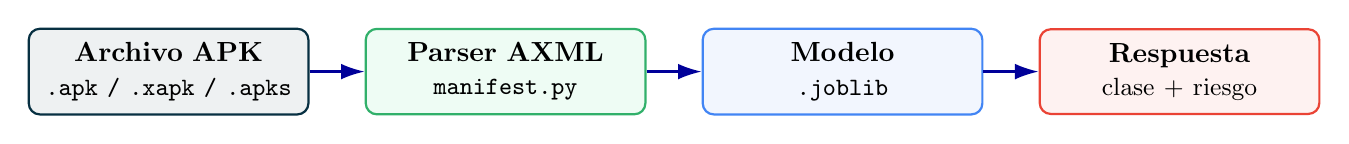
\begin{tikzpicture}[node distance=0.7cm]
    \node[compactapk, draw=androiddark, fill=androiddark!7] (apk) {
        \textbf{Archivo APK}\\
        \small \texttt{.apk / .xapk / .apks}
    };
    \node[compactapk, draw=androidgreen!80!black, fill=androidgreen!9, right=of apk] (parser) {
        \textbf{Parser AXML}\\
        \small \texttt{manifest.py}
    };
    \node[compactapk, draw=gcpblue, fill=gcpblue!7, right=of parser] (model) {
        \textbf{Modelo}\\
        \small \texttt{.joblib}
    };
    \node[compactapk, draw=gcpred, fill=gcpred!7, right=of model] (resp) {
        \textbf{Respuesta}\\
        \small clase + riesgo
    };

    \draw[flowarrow] (apk) -- (parser);
    \draw[flowarrow] (parser) -- (model);
    \draw[flowarrow] (model) -- (resp);
\end{tikzpicture}

\small\textbf{Figura:} Flujo de análisis de una APK real en la aplicación web.
\end{center}

El módulo \texttt{manifest.py} incluye un parser propio del formato AXML binario de Android que extrae permisos sin depender de herramientas externas como \texttt{aapt} ni del Android SDK.

\subsection{Ejecución de la aplicación}

Desde la carpeta raíz del proyecto:

\begin{lstlisting}
conda activate apk-malware
python -m frontend_webapp.app
\end{lstlisting}

Abra el navegador en:

\begin{lstlisting}
http://127.0.0.1:8001
\end{lstlisting}

La interfaz permite subir un archivo \texttt{.apk}, \texttt{.xapk} o \texttt{.apks} y muestra:

\begin{itemize}
    \item clase predicha (benigna / maliciosa);
    \item probabilidad de malware;
    \item score de riesgo (0--100);
    \item lista de permisos detectados;
    \item resultados por APK interno para contenedores \texttt{.xapk}.
\end{itemize}

\section{Predicción por línea de comandos}

Analice una APK directamente desde la consola:

\begin{lstlisting}
# Salida en texto legible
python -m frontend_cli.predict_apk testapk\homestar_apk.apk

# Salida estructurada en JSON
python -m frontend_cli.predict_apk testapk\WhatsApp.xapk --json

# Especificar un modelo alternativo
python -m frontend_cli.predict_apk ruta\archivo.apk \
    --model models/otro_modelo.joblib
\end{lstlisting}

Para entrenar un nuevo modelo desde el dataset:

\begin{lstlisting}
python -m frontend_cli.train_model \
    --data data/apk_train.csv \
    --output models/android_permission_best_model.joblib
\end{lstlisting}

El script entrena los tres modelos candidatos, selecciona el mejor por F1 sobre malware y guarda el artefacto \texttt{.joblib}.

\section{Conclusiones guiadas}

Al terminar de ejecutar el notebook completo, documente sus hallazgos respondiendo las siguientes preguntas:

\begin{enumerate}
    \item \textbf{H1:} ¿Los modelos supervisados superaron claramente la línea base mayoritaria? ¿Cuál fue la diferencia en F1 entre el mejor modelo y la línea base?
    \item \textbf{H2:} ¿El p-value de la prueba de Mann-Whitney permitió rechazar la hipótesis nula? ¿Cuántos permisos solicitan en promedio las APKs maliciosas frente a las benignas?
    \item \textbf{H3:} ¿Las APKs maliciosas tienen más permisos sensibles en promedio? ¿Cuáles son los tres permisos sensibles más frecuentes en malware?
    \item \textbf{H4:} ¿Cuántos permisos son exclusivos de cada clase y cuántos son compartidos? ¿Qué implica este solapamiento para la clasificación?
    \item \textbf{H5:} ¿Las reglas de clasificación con más de un permiso en el antecedente tienen mayor confianza que las reglas de un solo permiso?
    \item \textbf{H6:} ¿Con cuántos permisos el modelo reducido obtiene un F1 comparable al modelo completo?
    \item ¿Cuáles son los tres permisos más importantes según el mejor modelo? ¿Tienen sentido desde el dominio de seguridad en Android?
    \item ¿Qué limitaciones tiene el análisis estático por permisos para detectar malware sofisticado?
\end{enumerate}

\begin{tcolorbox}[title=Conclusión operativa]
Los permisos declarados en el manifiesto Android contienen información discriminativa real: los modelos supervisados alcanzan un desempeño muy superior a la línea base, los permisos sensibles son más frecuentes en malware, y un subconjunto reducido de permisos es suficiente para mantener un alto recall de malware. Sin embargo, el solapamiento entre clases confirma que los permisos no son una señal perfecta, y que el análisis estático debe complementarse con análisis dinámico para detectar malware que camufla su comportamiento.
\end{tcolorbox}

\end{document}
